\section{Materiais e métodos}

\subsection{Intel RAPL}
\begin{frame}{Intel RAPL}
    \begin{itemize}
        \item A
        \item B
        \item C 
        \item A
    \end{itemize}
\end{frame}

\begin{frame}{RAPL Power Domain}
    \begin{itemize}
        \item A
        \item B
        \item C 
        \item D 
    \end{itemize}
\end{frame}

\begin{frame}{Gerações E suporte ao RAPL dos Processadores Intel}
        \begin{figure}
            \centering
            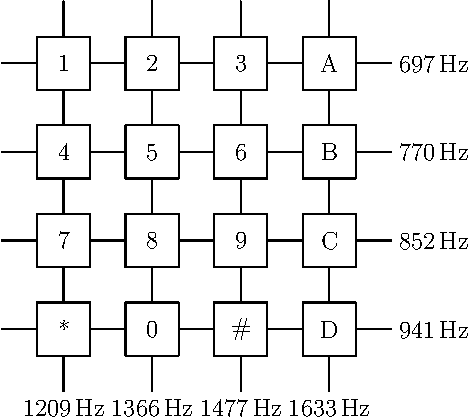
\includegraphics[width=0.35\linewidth]{images/dtmf.pdf}
            \caption{Exemplo de um PDF incluído em um frame}
            \label{fig:example}
        \end{figure}
\end{frame}

\subsection{GNU Time}
\begin{frame}{GNU Time}
    \begin{itemize}
        \item A
        \item B
        \item C 
        \item D 
    \end{itemize}
\end{frame}

\subsection{Shell}
\begin{frame}{Shell}
    \begin{itemize}
        \item A
        \item B
        \item C 
        \item Shell scripts
        \item Bash
    \end{itemize}
\end{frame}

\subsection{The Computer Language Benchmark Game}
\begin{frame}{The Computer Language Benchmark Game}
    \begin{itemize}
        \item A
        \item B
        \item C 
        \item D 
    \end{itemize}
\end{frame}
